\section{Esercitazione 2}
\subsection{Percettrone}
Un percettrone si basa su un’unica unità di calcolo che riceve un input e attraverso una funzione soglia valorizza l’uscita facendole assumere un valore 1 o -1.\\
Una rete neurale, e quindi anche l’unità di calcolo del percettrone, riceve in ingresso un segnale che viene scalato da alcuni pesi (parametri apprendibili dalla rete che devono essere fittati in modo corretto per diminuire la funzione di errore).\\

Il segnale di ingresso ha come prima componente un’unità che poi verrà scalata dal corrispettivo peso. 
La somma dei pesi moltiplicati per il segnale d’ingresso costituisce il potenziale di attivazione, dal quale viene determinato tramite la funzione a soglia il valore in output: se la sommatoria è maggiore di 0, l’output sarà 1, altrimenti -1. 
Nel percettrone, si considera come errore la differenza tra l’output (1 o -1) e il corrispettivo valore associato all’istanza in ingresso (label dell’esempio corrente).
L’errore viene poi fattorizzato nella variazione dei pesi $\Delta$ che viene sommata al peso attuale per generare il nuovo peso.

\begin{figure}[H]
    \centering
    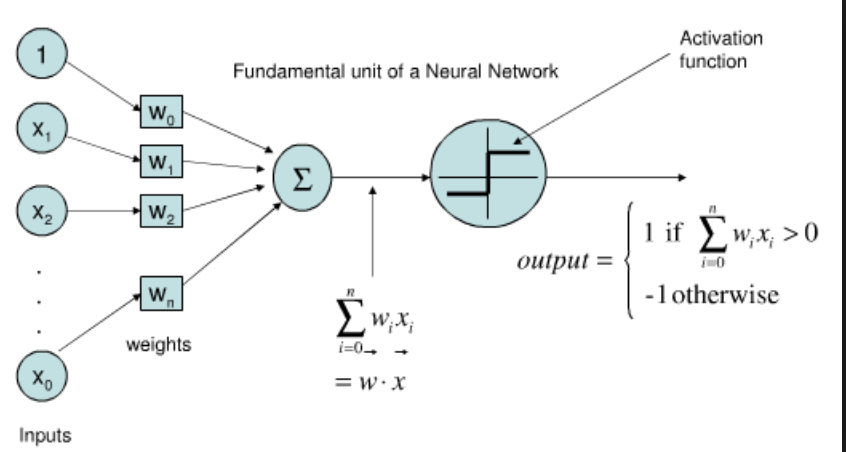
\includegraphics[scale = 0.8]{imm/perceptron_1.png}
\end{figure}

\textbf{Algoritmo}\\
Per esempio $(x,t)$ con $x$ istanza e $t$ etichetta target.
\begin{enumerate}
    \item Si computa $y = step(f(x))$
    \item  $w \leftarrow w + \alpha(t-y)x$, dove $\alpha$ è il learning rate
\end{enumerate}
Se l’output: 
\begin{itemize}
    \item corrisponde con il target: $(t-y) = 0$ e i pesi non vengono aggiornati 
    \item $=1$ e il target è $0$: l’input (scalato da $\alpha$) è sottratto dal vettore dei pesi.
    \item $=0$ e il target è $1$: l’input (scalato da $\alpha$) è aggiunto al vettore dei pesi.
\end{itemize}
\subsection{Adaline}

Simile al percettrone ma gli errori vengono valutati nel continuo (tramite una funzione di attivazione lineare che ha come argomento il potenziale).
Mentre nel percettrone l’output binario serviva per il calcolo dell’errore e l’aggiornamento dei pesi (per imparare i coefficienti del modello vengono usate le label); in Adaline l’errore viene calcolato su un valore continuo consentendo quindi di dire anche di quanto ci si è sbagliati (per imparare i coefficienti del modello si usano i valori continui predetti)
\begin{figure}[H]
    \centering
    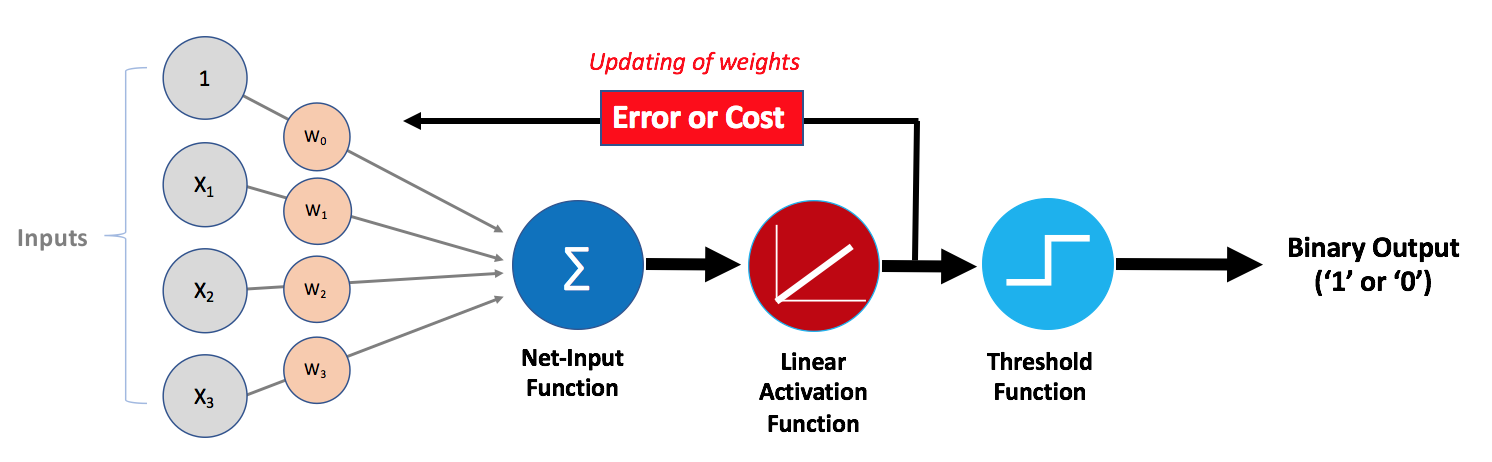
\includegraphics[scale = 0.5]{imm/perceptron_2.png}
\end{figure}

\textbf{Algoritmo}\\
Per esempio $(x,t)$ con $x$ istanza e $t$ etichetta target:
\begin{enumerate}
    \item Si computa $z = f(x)$
    \item  $w \leftarrow w + \alpha(t-z)x$, dove $\alpha$ è il learning rate
\end{enumerate}

Ciò equivale a applicare la regola del gradiente discendente alla regressione lineare (con lo squared error loss).
Infatti, la derivata di $(z-t)^2$ è $2(z-t)$ e il fattore costante $2$ può essere omesso dal momento che si sta usando $\alpha$ come learning rate per modulare quanto ogni update modifica i pesi correnti.

\begin{figure}[H]
    \centering
    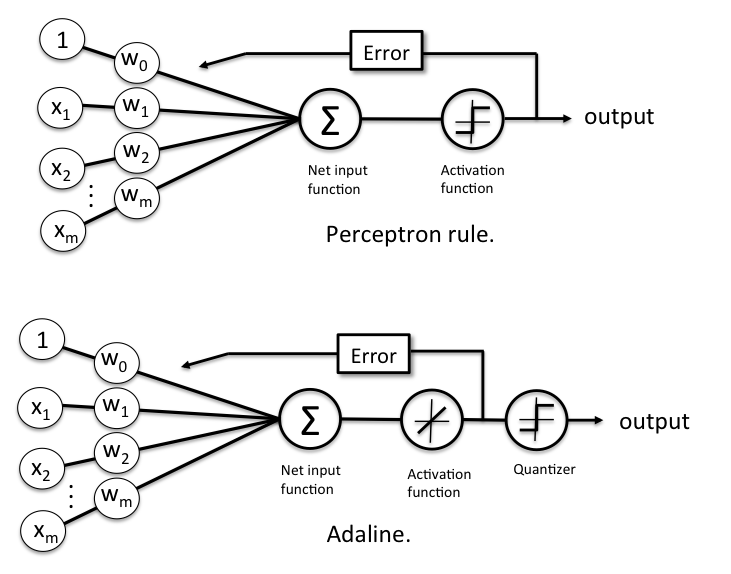
\includegraphics[scale = 0.8]{imm/perceptron_3.png}
\end{figure}

\begin{figure}[H]
    \centering
    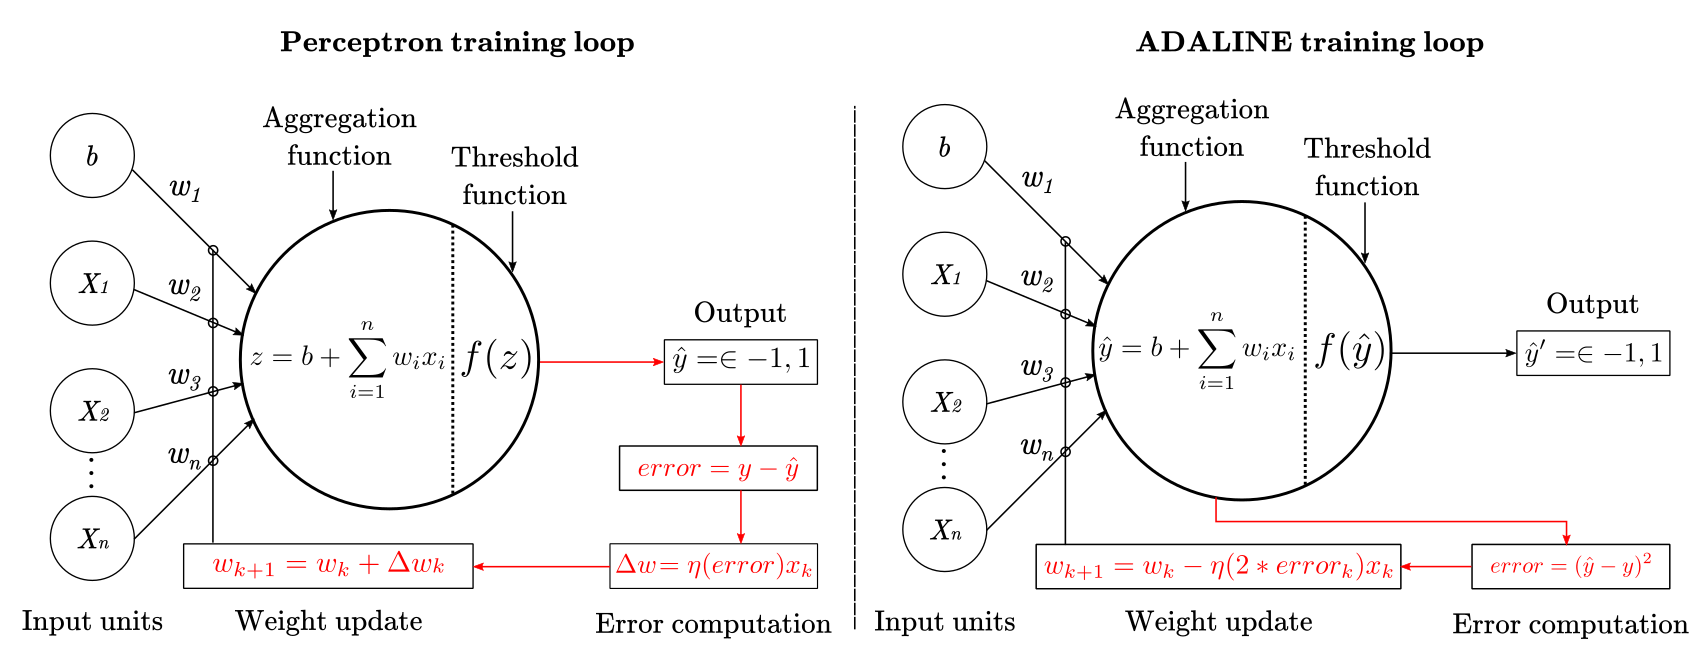
\includegraphics[scale= 0.6]{imm/adaline-math.png}
\end{figure}

\subsubsection{Separazione lineare}
Un set di punti linearmente separabili usa gli iperpiani per effettuare la separazione.

Le reti neurali dette feedforward neural networks prevedono diversi livelli computazionali: il segnale d’ingresso passa attraverso vari livelli (layers) in ognuno dei quali viene calcolata una funzione prendendo in input gli output della funzione del layer precedente.
